\section{Water}
The water is basically a squared plane (built in the same way of the flat terrain). Each cell has a water plane that will be visible only if some vertex of the cell has an height < of the water.

\begin{figure}[hbt!]
	\centering
	\subfloat[\centering Plane.]{{
\includegraphics[width=6.3cm]{images/Water.png}}}%
	\qquad
	\subfloat[\centering Vertices, indices and faces.]{{
\includegraphics[width=6.3cm]{images/WaterNoVert.png} }}%
	\caption{}
\end{figure}

\section{Reflection and refraction}
After creating the plane, the first thing I implemented was the reflaction and the refraction on the plane.

\subsubsection{Frame buffer objects}
The frame buffer is used to render our scene with all the information from the different buffers, such as color and depth. You can create your own frame buffer object to render the scene and save it in a texture. In particular, every time we render the scene in our frame buffer, we will update our 2D texture. This is exactly what we need because we need a texture to project inside the plane.
I'll quickly explain how I created the class for the frame buffer object (Full code in \textbf{waterFrameBuffer.h}).

\newpage

\noindent
First I defined a method to create the frame buffer using some OpenGL function.

\begin{figure}[hbt!]
	\centering
	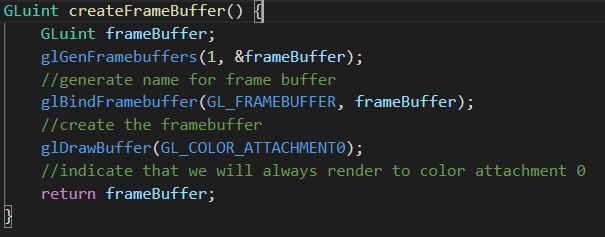
\includegraphics[width= 1
	\textwidth]{images/FBO1.png}
	\caption{Method for the creation of the frame buffer.}
\end{figure} 

\noindent
So I defined the two methods of creating texture attachment, one for colour and one for depth attachment. They are just a simple generation of a texture with a new "glFramebufferTexture" statement. (I only insert the screenshot of the attached colour since they are pretty much the same).

\begin{figure}[hbt!]
	\centering
	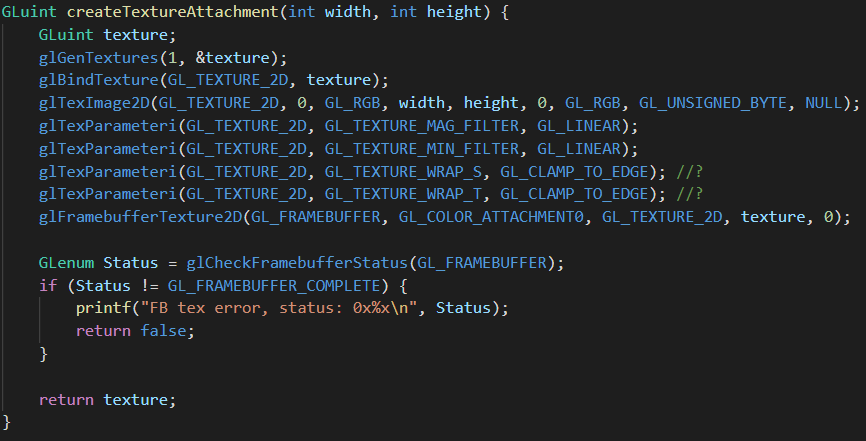
\includegraphics[width= 0.9
	\textwidth]{images/FBO2.png}
	\caption{Method for the creation of the texture.}
\end{figure} 

Last I defined a method to create the depth buffer. 

\begin{figure}[hbt!]
	\centering
	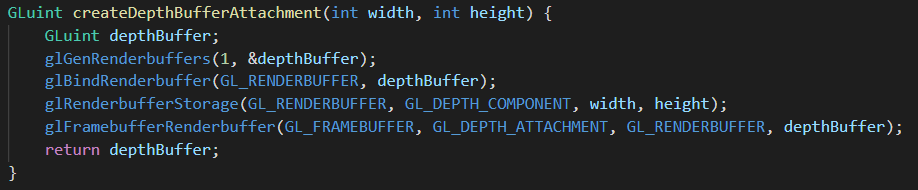
\includegraphics[width= 1
	\textwidth]{images/FBO4.png}
	\caption{Method for the creation of depth buffer.}
\end{figure} 

\noindent
Finally I created two methods, one to bind the frame buffer and one to unbind it so that I can switch from the normal frame buffer to the one created by me. I stored two frame buffers in this class, one for reflection and one for refraction. Basically I'll render the scene and create my own texture that will be used by the main render to apply it to the water.

\subsection{Clipping plane}
For both refraction and reflection textures, you don't need to render the whole scene. Actually I need the one above the surface for the reflection and the one under the water for refraction. So I defined the clipping plane which allowed me to render only a part of the scene and obviously it is positioned at the same level of the water. \\
After enabling a clipping plane (\textbf{glEnable(GL\textunderscore CLIP \textunderscore DISTANCE0)}) in the main rendering, I use the \textbf{gl\textunderscore ClipDistance[0]} variable in the shaders to define which vertex should be clipped. If this distance is positive, I should render this vertex, if negative no. To calculate it, I simply use the dot product of the world position (model matrix * position) and the horizontal plane, whose equation is \textbf{vec4}(0, -1/+1, waterHeight). The Y component will be +1 if we want to clip the lower part (reflection) or -1 if we want to clip the upper part (refraction)

\newpage

\begin{figure}[hbt!]
	\centering
	\subfloat[\centering Clipping the below part.]{{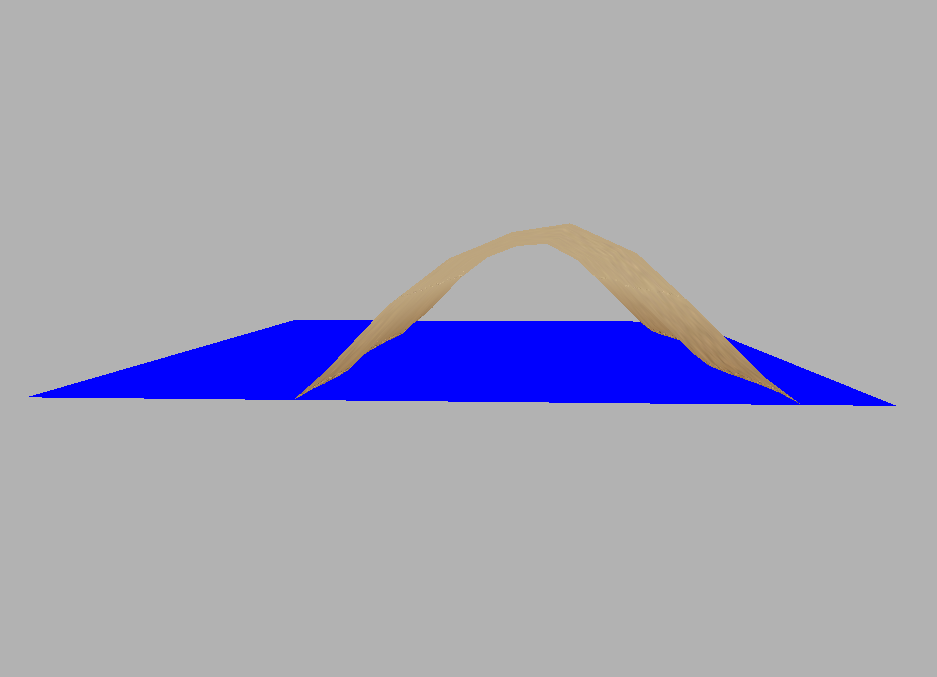
\includegraphics[width=6.3cm]{images/Water1.png}}}%
	\qquad
	\subfloat[\centering Clipping the above part.]{{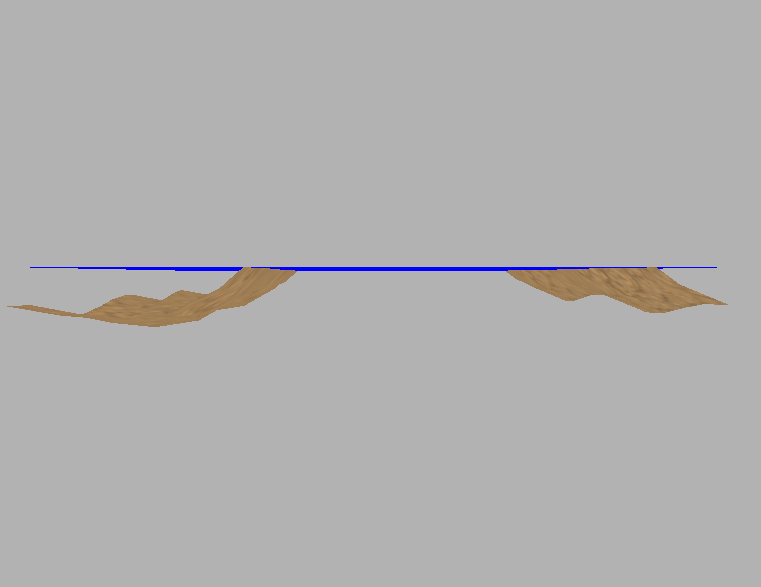
\includegraphics[width=6.3cm]{images/Water2.png} }}%
	\caption{}
\end{figure}

\subsection{Projective texture mapping}
To apply the texture to the plane, I used \textbf{projective texture mapping} that is a texture mapping method that allows you to project a textured image onto a scene. I needed to find the correct UV coordinate and for that I just found the screen space coordinate on the water coordinates and I can use those exactly to sample the texture. Basically I need to calculate the normalized device coordinates and I can do it using the perspective division. I just need to divide the clip space component (projection matrix * view matrix * model matrix * position) into its \textbf{W} component and then divide by 2 and add 0.5 to find the correct coordinate system .

\begin{equation}
newCoord = vec2(clipspace.xy / clipspace.w) 2.0 + 0.5)		
\end{equation}

\noindent
Now I can sample the refraction and the reflection by using the X and Y components as texture coordinates.
I also need to mention that the rendering for the reflection texture is done with the camera reversed and shifted slightly down to give the reflection effect. On the other hand, no changes are applied to refraction rendering.

\newpage

\begin{figure}[hbt!]
	\centering
	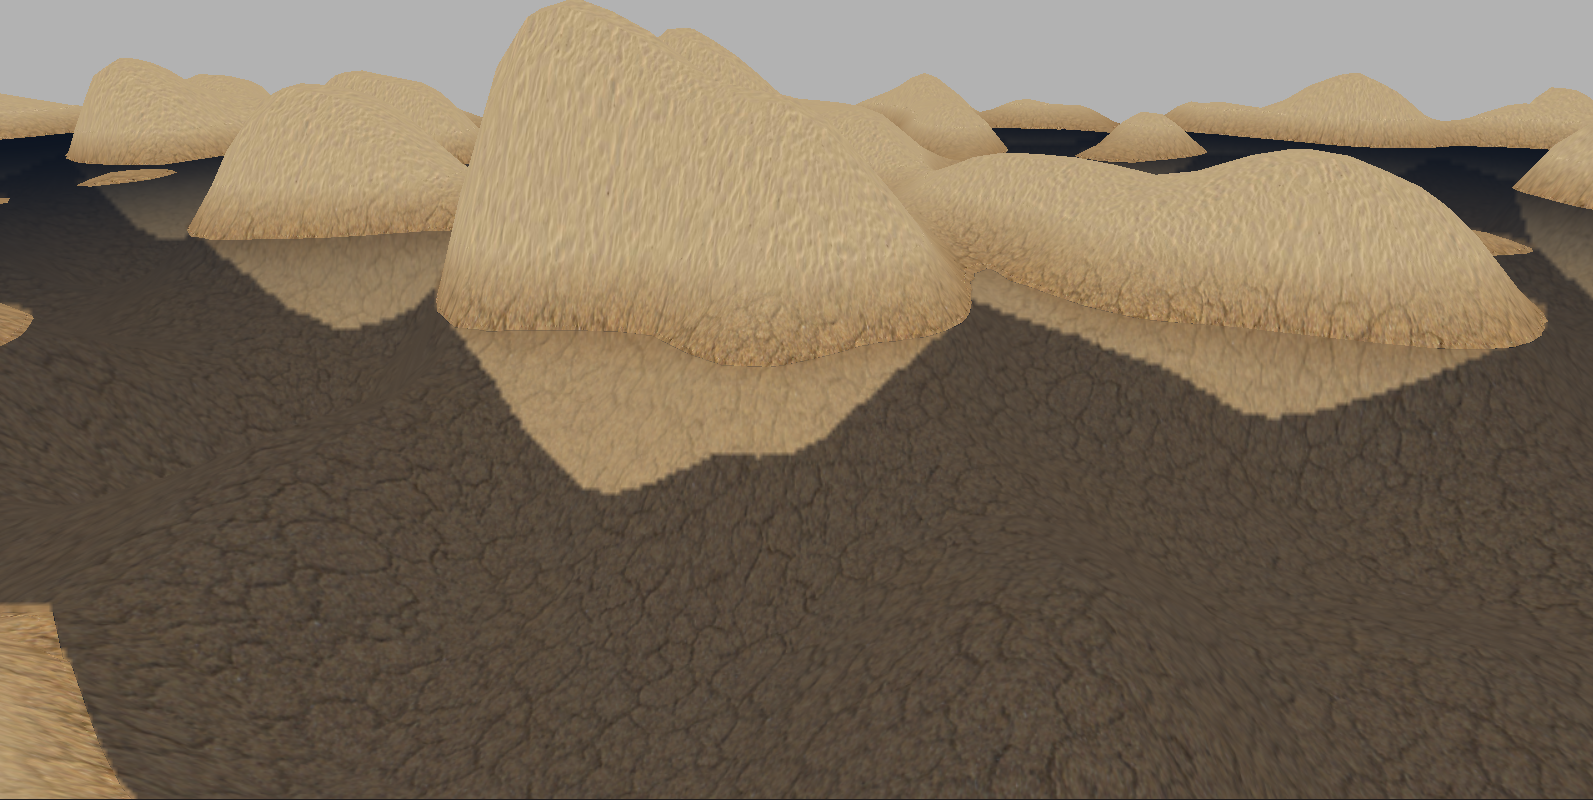
\includegraphics[width= 1
	\textwidth]{images/Water3.png}
	\caption{Reflection and Refraction texture mixed.}
\end{figure} 